\chapter[综合案例一：地铁客流预测全流程]{综合案例一：地铁进站客流预测的全流程协作}
\label{ch:case_one}

第 15 章用贯穿案例 C 走读了一个完整项目的骨架。本章把这个项目完整展开：从项目章程出发，经过数据理解、清洗、特征工程、基准与建模、验证、边界识别，直到交付与监控。与前面各章的案例不同，本章不再聚焦于某一个知识点，而是展示 Prompting、Modeling 与 Evaluation 如何在同一个项目中反复交替。

本章使用的全部数据都是真实的公开数据：纽约大都会运输署（MTA）在纽约州开放数据平台发布的地铁分小时进站客流\cite{mta2025hourly}、美国职业棒球大联盟（MLB）官方赛程接口提供的主场比赛时间，以及 Open-Meteo 提供的纽约逐日天气实测与历史预报。需要说明的是，项目本身是为教学而设计的：书中的“项目组”“章程”和“决策”是按照真实项目的工作方式组织的，并不代表 MTA 实际开展过这一项目；但书中报告的每一个数据现象和数值结果，都由配套代码 \texttt{code/case\_C\_metro/} 在真实数据上实际运行得到。

本章的每一节都遵循相同的结构：这一阶段要回答的问题是什么；向 AI 提交了什么 Prompt；AI 给出了什么；人做了哪些检查和决定。

\begin{chapterguide}
\begin{itemize}
  \item 将前面各章的方法组织成一个连贯的项目流程；
  \item 在每个阶段识别哪些工作可以交给 AI，哪些决策必须由人完成；
  \item 设计贯穿全项目的公共上下文，使多轮 AI 协作保持一致；
  \item 把验证结果转化为交付形式、使用边界和监控方案。
\end{itemize}
\end{chapterguide}

% ----------------------------------------------------------------
\section{项目背景与公共上下文}
% ----------------------------------------------------------------

\subsection{项目章程摘要}

纽约地铁 24 小时运营，MTA 按“车站综合体”（station complex）逐小时公布进站量，并区分 MetroCard 磁卡和 OMNY 非接触支付两种方式。本项目选取 9 座特点各异的车站：时代广场、中央车站、富尔顿街三座曼哈顿大型枢纽；巴克莱中心（大西洋大道）；扬基体育场（161 街）与大都会队主场（Mets-Willets Point）两座球场车站；以及法拉盛主街、杰克逊高地、上东区 86 街三座以居住和通勤为主的车站。

项目一期的章程要点如下：

\begin{description}
  \item[目标] 每天 16:00 输出次日各车站 5:00—23:00 每小时的进站量预测，供车站排定次日站务与引导人员。
  \item[成功标准] 在测试期内，加权 MAE 明显低于“近四周同日同时段均值”基准；非常规日（节假日前后、球场比赛日）的改进不低于常规日。
  \item[错误成本] 早晚高峰（7:00—9:59、17:00—19:59）以及三座大型枢纽，低估误差的权重为 2，其余为 1。
  \item[非目标] 不做实时限流；不决定列车运行计划；不自动生成排班方案。
  \item[停止条件] 若在验证期内无法稳定优于基准，项目停止在“基准 + 人工经验”方案。
\end{description}

\subsection{贯穿全项目的公共上下文}

一个跨越多周、包含数十轮 AI 对话的项目，最大的风险之一是上下文漂移：前面确认过的定义，在后面的对话中被 AI 按照默认假设悄悄替换。项目组把章程、数据字典和关键约束整理成一份“公共上下文”，作为每一轮新对话的开头：

\begin{quote}
\textbf{【公共上下文 v1.2，每次对话开头提供】}

\textbf{项目：}纽约地铁 9 座车站次日分小时进站量预测（一期，服务于站务排班）。

\textbf{分析单元与标签：}车站综合体 $\times$ 小时；标签为该小时的进站量 = MetroCard 进站 + OMNY 进站。缺失的小时保持缺失，不得填为 0。

\textbf{预测时刻与信息可得性：}预测在 $D-1$ 日 16:00 做出。可用信息：$D-2$ 日及以前的完整客流数据，以及 $D-7$、$D-14$、$D-21$、$D-28$ 日的同小时客流；日历与联邦节假日；已公布的 MLB 主场赛程；$D-1$ 日可得的次日天气预报。\textbf{不可用}：$D$ 日及之后的任何实测数据，包括实测天气。

\textbf{数据划分（已冻结）：}训练 2022-03-01—2023-12-31；验证 2024-01-01—2024-03-31；测试 2024-04-01—2024-06-30。

\textbf{评价：}主指标为加权 MAE（权重规则见章程）；同时按日期类型（常规工作日、周末、节假日前后、球场比赛日）和车站分别报告；必须与两个基准比较。

\textbf{协作规则：}每一步先输出计划，经确认后再实现；任何对上述定义的偏离都必须显式说明；不确定时停止并提问。
\end{quote}

这份文件在项目中经历了多次版本更新，每一次更新都对应一项被记录的决策变化。把它称为“代码”并不夸张：它被版本管理，被每一轮协作“调用”，一旦出错，后续所有结果都会随之出错。

% ----------------------------------------------------------------
\section{数据理解：先描述，再清洗}
% ----------------------------------------------------------------

\subsection{让 AI 先描述数据}

项目组通过开放数据平台的接口，按车站和月份下载了 2022 年 2 月至 2024 年 12 月的分小时数据（下载脚本见 \texttt{code/case\_C\_metro/fetch\_mta.py}）。随后向 AI 提交了第一个分析请求：

\begin{quote}
【公共上下文】

\textbf{本步骤任务：}读取 \texttt{mta\_hourly\_selected.csv}，暂时不要做任何清洗或删除。请输出：(1) 每座车站的记录数与时间范围；(2) 按月汇总的进站量，分 MetroCard 与 OMNY 两种支付方式分别统计，并计算 OMNY 占比；(3) 把每座车站补全为完整的小时序列后，缺失的小时数及其集中的日期；(4) 日进站量低于该站中位数 30\% 的“车站—日”。请只描述发现，不要给出任何处理建议。
\end{quote}

“只描述发现，不要给出处理建议”这一句是有意为之。数据理解阶段最常见的问题，是 AI 在发现异常的同时就给出处理方案，而使用者在未理解异常原因之前就接受了方案。把“描述”与“决策”分开，是第 5 章“决策在人，实现在 AI”原则的直接体现。

\subsection{四个发现}

\paragraph{发现一：支付方式在迁移} 9 座车站合计的 OMNY 占比从 2022 年 2 月的 27.9\% 持续上升，到 2024 年 11 月达到 65.6\%。如果只看 MetroCard 数据，2022 年 3 月至 2024 年 11 月的月进站量下降了 35.0\%；而把两种支付方式相加，同期总进站量实际上升了约 33\%。任何只使用其中一种支付方式的数据，都会得出与现实方向相反的趋势。图~\ref{fig:ch16_payment} 展示了这一点。

\begin{figure}[H]
  \centering
  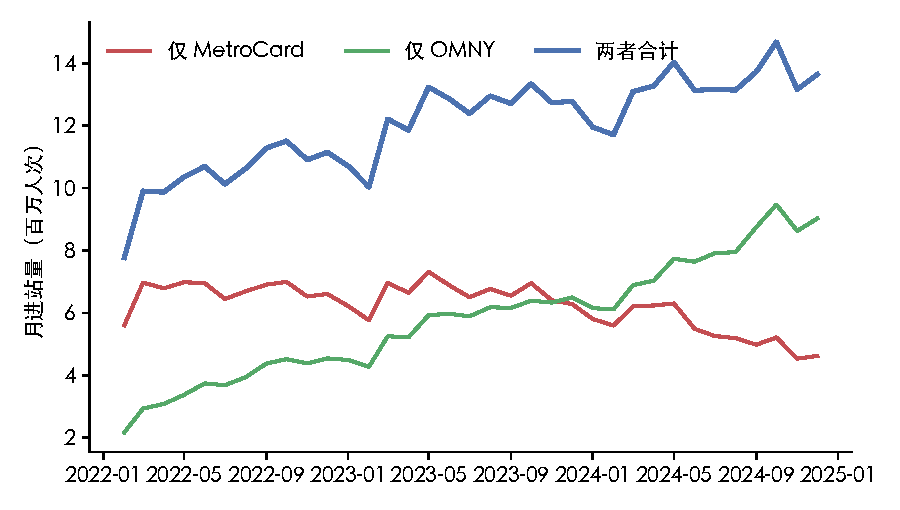
\includegraphics[width=0.8\textwidth]{figures/chapter16/payment_trend.pdf}
  \caption{案例 C：9 座车站的月进站量，按支付方式分别统计与合计}
  \label{fig:ch16_payment}
\end{figure}
这也是第 15 章所述“数据探索改变标签定义”的真实版本：标签必须定义为两种支付方式之和。

\paragraph{发现二：缺失的小时集中在夏令时切换日} 补全完整小时序列后，共有 218 个“车站—小时”缺失，仅占 0.09\%。但它们的分布很有规律：2022 年 3 月 13 日、2023 年 3 月 12 日、2024 年 3 月 10 日都在其中——这些正是美国夏令时开始的日期，当天凌晨 2 点这一小时在本地时间中并不存在。另有一部分缺失集中在 2023 年 2 月至 3 月的若干个周末。前者是时间表示问题，后者需要结合当时的施工与停运通告核实。无论哪一种，都不能用 0 填补。

\paragraph{发现三：异常低客流日有明确的日历含义} 日进站量低于中位数 30\% 的“车站—日”共 29 个，集中在圣诞节（2022、2023、2024 年的 12 月 25 日）、感恩节，以及 2022 年初的若干周末。它们是真实的低客流，而不是数据错误，应当作为节假日效应保留。

\paragraph{发现四：球场车站的客流高度依赖比赛} 在 2022—2024 年的数据中，扬基体育场车站在有主场比赛的日子，5:00—23:00 的小时平均进站量约为 1,256 人次，是无比赛日（约 635 人次）的近 2 倍；大都会队主场车站的差别更大，分别约为 572 和 164 人次，相差约 3.5 倍。对这两座车站而言，“当天有没有比赛、几点开赛”几乎决定了客流的形态。

\subsection{人的判断}

每一个发现都需要人去解释，而且解释依赖于 AI 无法从数据本身获得的信息：支付方式迁移需要知道 OMNY 的推广进程；夏令时缺失需要知道美国的时间制度；异常低客流需要对照节假日历；球场客流需要知道赛程。项目组据此确定了清洗规则（表~\ref{tab:ch16_cleaning}），完整实现见 \texttt{code/case\_C\_metro/step1\_clean.py}。

\begin{table}[H]
\centering
\caption{案例 C：清洗规则表}
\label{tab:ch16_cleaning}
\small
\begin{tabular}{p{0.6cm}p{5.6cm}p{3.6cm}p{2.4cm}}
\toprule
编号 & 规则 & 依据 & 处理 \\
\midrule
C1 & 标签 = MetroCard 进站 + OMNY 进站 & 支付方式迁移 & 合并 \\
C2 & 补全完整的小时索引，缺失小时保持为缺失 & 缺失不等于零客流 & 标记缺失 \\
C3 & 夏令时切换造成的缺失小时，不做插补 & 该小时在本地时间中不存在 & 保持缺失 \\
C4 & 节假日等真实低客流日全部保留 & 日历效应是真实信号 & 保留 \\
C5 & 不删除任何高客流记录 & 比赛散场等高峰是排班重点 & 保留 \\
\bottomrule
\end{tabular}
\end{table}

规则 C5 值得特别说明。如果按照“超过均值加 3 倍标准差即为异常”的常规做法，球场车站的比赛散场时段几乎都会被识别为异常值——而这些时段恰恰是站务排班最需要关注的时刻。这与第 5 章讨论的暴雨天气出行需求峰值是同一类问题：统计上的异常，不等于业务上的错误。

% ----------------------------------------------------------------
\section{特征工程：把运营知识变成特征}
% ----------------------------------------------------------------

\subsection{特征的来源}

项目组先列出了一份“特征假设清单”，每一项都写明它所编码的现实机制，再让 AI 实现：

\begin{description}
  \item[周期性] 小时、星期几、月份；$D-7$、$D-14$、$D-21$、$D-28$ 日同小时进站量及其均值。
  \item[日历效应] 是否联邦节假日、距最近节假日的天数（截断为 7）。
  \item[大型活动] 球场车站当天是否有主场比赛，以及当前小时距开赛的小时数。赛程在比赛前早已公布，满足信息可得性。
  \item[天气] 次日降水量与最高气温。提供实测与预报两个版本，用于检验信息可得性的影响。
  \item[近期趋势] 最近 7 个完整日（$D-8$ 至 $D-2$）同小时均值与更早 28 天均值之比，用于捕捉季节变化和支付迁移之外的缓慢趋势。
\end{description}

不同类型车站的客流规律差异很大，这也是特征需要按车站区分的原因。图~\ref{fig:ch16_profiles} 比较了三座车站工作日的日内分布：中央车站是典型的通勤枢纽，晚高峰占比最高；法拉盛主街以早高峰出发为主；扬基体育场车站则在 21—22 时出现了一个其他车站没有的高峰，对应夜场比赛的散场。

\begin{figure}[H]
  \centering
  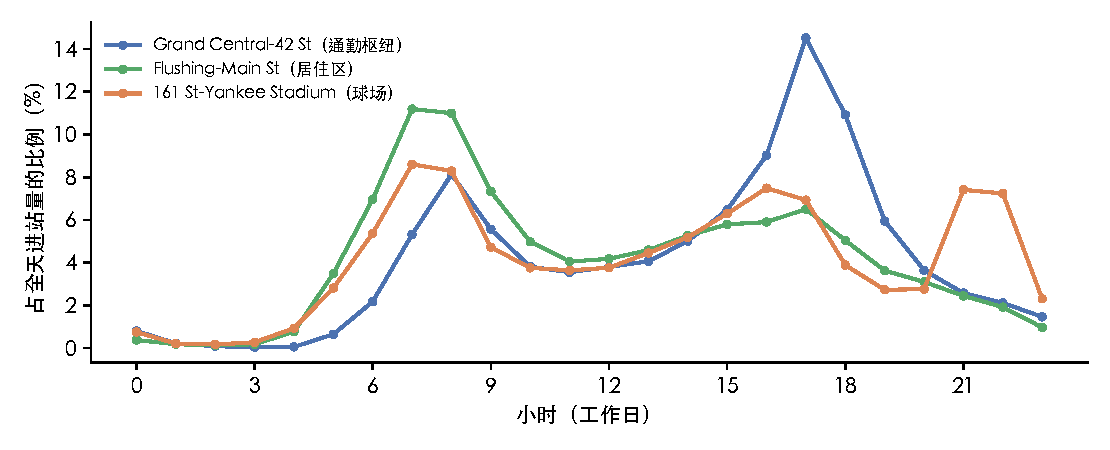
\includegraphics[width=0.9\textwidth]{figures/chapter16/station_profiles.pdf}
  \caption{案例 C：三类车站工作日的日内进站分布（2022—2024 年平均）}
  \label{fig:ch16_profiles}
\end{figure}

\subsection{防泄露约束与代码审查}

\begin{quote}
【公共上下文】

\textbf{本步骤任务：}按照“特征假设清单”构造特征。

\textbf{特别约束：}
\begin{enumerate}
  \item 所有基于历史客流的特征，计算窗口必须严格位于 $D-2$ 日及以前，或为 $D-7k$ 日同小时；
  \item 缺失标签在计算历史均值时应被跳过，而不是作为 0 参与计算；有效值少于 2 个时，特征置为缺失；
  \item 请为每个特征函数写一个单元测试：构造包含 2 座车站、10 个运营日的小样本，人工计算期望值，验证函数输出。
\end{enumerate}
\end{quote}

AI 生成的核心函数如代码清单~\ref{lst:ch16_lag} 所示。

\begin{lstlisting}[caption={案例 C：同日同小时历史特征的构造},label={lst:ch16_lag}]
def add_weekly_lags(df, lags=(7, 14, 21, 28)):
    """按日期平移后合并，而不是 shift(k)：即使某些行不存在也不会错位。"""
    base = df[["station", "date", "hour", "entries"]]
    for k in lags:
        s = base.copy()
        s["date"] = s["date"] + pd.Timedelta(days=k)
        df = df.merge(s.rename(columns={"entries": f"lag_{k}d"}),
                      on=["station", "date", "hour"], how="left")
    cols = [f"lag_{k}d" for k in lags]
    df["mean_4w"] = df[cols].mean(axis=1, skipna=True)
    df.loc[df[cols].notna().sum(axis=1) < 2, "mean_4w"] = np.nan
    return df
\end{lstlisting}

这段代码采用“把历史表的日期向后平移 $k$ 天再按键合并”的方式，而不是 \texttt{shift(k)}。项目组在审查时特意确认了这一点：如果某些“车站—日期—小时”的行不存在，\texttt{shift} 会按行数而非日期偏移，从而悄悄错位；按日期合并的写法对这种情况是稳健的。近期趋势特征则使用了 \texttt{rolling(...).shift(2)}，审查者逐行核对了 \texttt{shift(2)} 确实保证窗口截止于 $D-2$ 日。完整实现见 \texttt{code/case\_C\_metro/step2\_features.py}。

在准备外部数据时，还出现了一个值得记录的小插曲：AI 编写的赛程下载函数一次性请求 2022—2024 年的 MLB 赛程，返回结果中只有一个赛季的比赛（扬基队共 94 场主场）。项目组对照“每个赛季约 81 场常规赛主场”的常识，立即发现数量不对；改为逐赛季请求后，得到三个赛季共 267 场扬基队主场和 265 场大都会队主场比赛（含季后赛）。这是一个典型的“代码能运行、结果不报错、但数量级不对”的错误，它是被领域常识而不是测试捕获的。

% ----------------------------------------------------------------
\section{基准与建模}
% ----------------------------------------------------------------

\subsection{先建立基准}

按照章程，项目组首先实现了两个基准：B1“上周同日同时段”和 B2“近四周同日同时段均值”。

\subsection{模型选择与加权损失}

\begin{quote}
【公共上下文】

\textbf{本步骤任务：}在基准之上训练预测模型。请先提出 2—3 种候选方案，比较它们在本项目中的适用性，重点考虑：(1) 9 座车站的客流规模相差二十余倍；(2) 两座球场车站的客流高度依赖比赛；(3) 需要输出预测区间；(4) 章程中的非对称错误成本。暂时不要实现。
\end{quote}

AI 提出了为每座车站单独建模、所有车站共享一个全局梯度提升树模型、以及时序神经网络三种方案。项目组选择了全局梯度提升树，理由是：全局模型可以让不同车站共享日历和天气效应，同时通过车站类别特征保留各站差异；树模型对缺失特征的处理较为自然；训练成本低，便于每月重训。预测区间通过分别训练 10\% 和 90\% 分位数模型获得。

章程中“低估误差权重为 2”的要求，需要同时体现在评价和训练中。项目组训练了两个版本：一个以 MAE（绝对误差）为损失；另一个以 2/3 分位数损失为目标——在分位数损失下，把低估的代价设为高估的 2 倍，最优预测恰好是条件分布的 2/3 分位数。评价使用的加权 MAE 如代码清单~\ref{lst:ch16_wmae} 所示。

\begin{lstlisting}[caption={案例 C：按章程定义的加权 MAE},label={lst:ch16_wmae}]
def weighted_mae(y, p, peak, top):
    err = p - y
    w = np.where((err < 0) & (peak | top), 2.0, 1.0)  # 高峰或大站的低估加倍
    m = ~np.isnan(y) & ~np.isnan(p)                   # 缺失标签不参与评价
    return float(np.sum(w[m] * np.abs(err[m])) / np.sum(w[m]))
\end{lstlisting}

\subsection{结果}

表~\ref{tab:ch16_results} 给出了测试集上的主要结果（完整代码见 \texttt{code/case\_C\_metro/step3\_models.py}）。

\begin{table}[H]
\centering
\caption{案例 C：测试集（2024 年 4—6 月）上的加权 MAE（人次/小时）}
\label{tab:ch16_results}
\small
\begin{tabular}{lccccc}
\toprule
方法 & 总体 & 常规工作日 & 周末 & 节假日前后 & 球场比赛日 \\
\midrule
B1 上周同日 & 344.4 & 320.0 & 275.0 & 540.0 & 576.4 \\
B2 近四周均值 & 270.2 & 235.9 & 218.2 & 504.4 & 502.6 \\
GBDT（实测天气） & 230.6 & 213.3 & 189.1 & 393.5 & 344.2 \\
GBDT（预报天气） & 227.7 & 210.5 & 190.9 & 370.5 & 340.6 \\
GBDT（预报天气，2/3 分位数损失） & 229.4 & 208.3 & 206.1 & 350.2 & 346.1 \\
\bottomrule
\end{tabular}
\end{table}

使用预报天气的 GBDT 模型总体比 B2 降低约 16\%；在节假日前后和球场比赛日，改进幅度分别约为 27\% 和 32\%，满足“非常规日改进不低于常规日”的要求。几个细节值得注意：

\begin{itemize}
  \item \textbf{实测天气并没有带来优势。} 在本案例中，使用实测天气（不可用）与使用预报天气（可用）的模型表现几乎相同，在实测与预报降水相差超过 10 mm 的 6 个测试日上，预报天气模型的 MAE（241.2）甚至低于实测天气模型（249.2）。这说明信息泄露并不总是造成明显的虚高——但它仍然是方法上的错误，必须修正，因为下一次它可能造成严重的虚高。
  \item \textbf{2/3 分位数损失改变了误差结构。} 它在常规工作日和节假日前后降低了加权 MAE（因为这些时候的低估代价被放大），却在周末提高了误差。损失函数不是“越复杂越好”，而是在不同日期类型之间重新分配误差；是否采用，应当回到章程中的错误成本来决定。
  \item \textbf{验证集与测试集的一致性。} 在验证集（2024 年 1—3 月）上，B2 与 GBDT（预报天气）的加权 MAE 分别为 302.8 和 244.5，改进幅度与测试集接近，说明模型选择没有过度依赖某一段时间。
\end{itemize}

% ----------------------------------------------------------------
\section{验证：按第 13 章的流程逐项检查}
% ----------------------------------------------------------------

模型结果满足成功标准，并不意味着验证已经完成。项目组按照第 13 章的流程逐项检查，完整脚本见 \texttt{code/case\_C\_metro/step4\_validate.py}。

\paragraph{量纲与数量级检查} 测试集中没有预测值超过该站该小时训练期最大值的 1.5 倍，但有 14 个预测值为负数，集中在扬基体育场车站的 23 时和大都会队主场车站的非比赛时段。进站量不可能为负。原因是梯度提升树的叶节点输出是残差修正的累加，在低客流时段可能越过 0。修正方法是对输出截断至 0，并在模型卡中记录这一现象。这是一个 AI 在报告中完全没有提及、却被最简单的合理性检查拦下的问题。

\paragraph{分车站检查} 按车站计算的相对误差（MAE 除以平均小时进站量）差异很大：时代广场、法拉盛主街等车站约为 6\%—8\%；巴克莱中心约为 12\%；扬基体育场约为 27\%；大都会队主场约为 53\%。相对误差最高的两座都是球场车站，巴克莱中心则是 NBA 布鲁克林篮网队主场和大量演唱会的举办地，而这些活动并未纳入本期的活动特征——这是一个需要在下一期补充数据来验证的假设。

\paragraph{极端情景检查：比赛散场} 项目组要求 AI 把扬基体育场和大都会队主场车站的比赛日误差，按“距开赛的小时数”展开（表~\ref{tab:ch16_game}）。

\begin{table}[H]
\centering
\caption{案例 C：球场车站比赛日按距开赛小时数的误差（测试集，人次/小时）}
\label{tab:ch16_game}
\begin{tabular}{lccc}
\toprule
距开赛小时数 & 实际平均进站量 & GBDT 平均偏差 & B2 平均偏差 \\
\midrule
$-1$ & 434 & $-26$ & $+22$ \\
0 & 409 & $-38$ & $+68$ \\
$+1$ & 748 & $-107$ & $-303$ \\
$+2$ & 3,968 & $-1,597$ & $-2,820$ \\
$+3$ & 4,559 & $-863$ & $-3,352$ \\
$+4$ & 1,082 & $-227$ & $-654$ \\
\bottomrule
\end{tabular}
\end{table}

\begin{figure}[H]
  \centering
  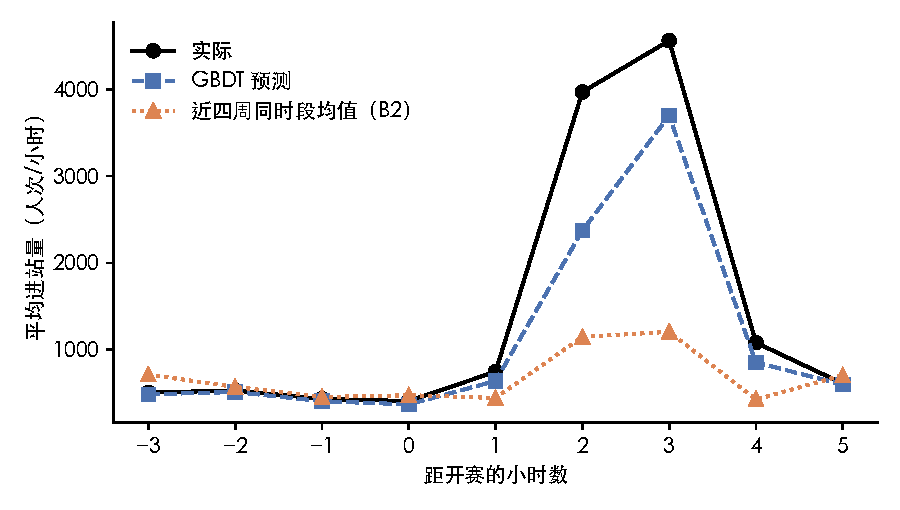
\includegraphics[width=0.75\textwidth]{figures/chapter16/game_profile.pdf}
  \caption{案例 C：球场车站比赛日按距开赛小时数的平均进站量（测试集）}
  \label{fig:ch16_game}
\end{figure}

图~\ref{fig:ch16_game} 直观地展示了这一差距。比赛通常在开赛后约 2.5 至 3 小时结束，散场时段（开赛后 2—3 小时）的平均进站量是赛前的 8 至 10 倍。模型已经大幅改进了基准——B2 完全不知道当天有比赛，偏差接近实际值本身——但在开赛后第 2 小时，模型仍然平均低估约 1,600 人次，约为实际值的 40\%。原因之一是比赛时长并不固定，散场高峰落在第 2 小时还是第 3 小时取决于比赛进程，而这在前一天是无法知道的。这个发现直接影响了交付形式：对于比赛日散场时段，与其给出一个单一数值，不如提示“散场高峰可能出现在 21:00—23:00 之间，峰值约为平日的 8 至 10 倍”。

\paragraph{预测区间检查} 名义上的 80\% 预测区间，在测试集上的实际覆盖率只有 74.3\%，在节假日前后为 69.0\%，在球场比赛日为 71.4\%。区间偏窄，意味着模型对自身不确定性的估计过于乐观，尤其是在非常规日。在交付前，项目组用验证集对区间做了经验校准（按日期类型放宽区间宽度），并把“区间覆盖率”列为上线后的监控指标之一。

图~\ref{fig:ch16_cov} 汇总了预测区间检查和分车站检查的结果。两张图指向同一个结论：模型在常规日表现稳定，而误差和不确定性都集中在比赛和节假日这类“非常规日”。

\begin{figure}[H]
  \centering
  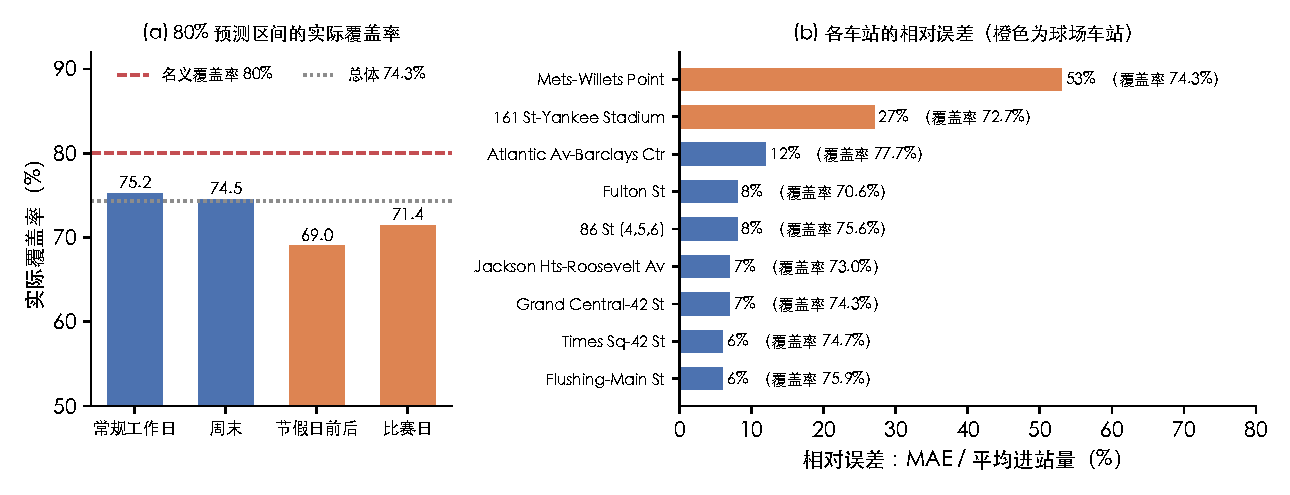
\includegraphics[width=\textwidth]{figures/chapter16/coverage.pdf}
  \caption{案例 C：预测区间的实际覆盖率与各车站的相对误差（测试集）}
  \label{fig:ch16_cov}
\end{figure}

\paragraph{反向追问} 项目组把完整的方法说明和结果交给另一个 AI 会话，要求它“扮演一位对数据泄露和评价偏差特别敏感的审稿人，列出至少 5 个可能导致测试结果偏乐观的原因，并说明如何检验”。这类审查中最有价值的，往往是那些此前没有想到的问题。例如：“测试期只有 2024 年第二季度，恰逢棒球赛季，结论能否推广到冬季？”这一问题提示项目组在模型卡中写明评价期的季节局限，并用 2024 年第四季度数据补充评估（读者可以用配套代码自行完成这一扩展）。

% ----------------------------------------------------------------
\section{边界识别：AI 在这个项目中扮演什么角色}
% ----------------------------------------------------------------

按照第 14 章的框架，项目组对 AI 参与的各个环节逐一确定了角色（表~\ref{tab:ch16_roles}）。

\begin{table}[H]
\centering
\caption{案例 C：AI 在项目各环节中的角色}
\label{tab:ch16_roles}
\small
\begin{tabular}{p{3.0cm}p{2.0cm}p{7.6cm}}
\toprule
环节 & AI 角色 & 说明 \\
\midrule
数据下载与描述 & 执行者 & 输出可以被逐项核对；描述与决策分离 \\
清洗规则实现 & 执行者 & 规则由人制定，AI 实现并报告影响量 \\
特征设计 & 副驾驶 & AI 可以补充候选特征，入选与否由人根据机制判断 \\
模型方案选择 & 副驾驶 & AI 比较候选方案，人结合车站差异与错误成本做决定 \\
每日预测运行 & 执行者 & 自动运行，但受监控和回退规则约束 \\
比赛散场、恶劣天气 & 参谋 & 模型给出提示和区间，由站务人员结合现场信息决定 \\
排班决定 & 不参与 & 预测只是排班的输入之一，排班由车站管理人员决定 \\
\bottomrule
\end{tabular}
\end{table}

最后一行“不参与”并非对 AI 能力的否定。排班涉及员工的工作时间、临时调配、现场突发情况和劳动规定，这些因素既不在数据中，也不应由模型决定。把预测与决策分开，也使责任边界清晰。

% ----------------------------------------------------------------
\section{交付、模型卡与监控}
% ----------------------------------------------------------------

\subsection{交付形式}

最终的每日报告包含三个部分：

\begin{enumerate}
  \item 次日 5:00—23:00 每小时的预测值与经过校准的 80\% 预测区间；
  \item 相对近四周同日均值偏差超过 15\% 的时段高亮，并附主要原因（如“联邦节假日前一天”“扬基队主场 19:05 开赛”“预报降水 20 mm 以上”），原因由固定模板根据特征生成；
  \item 不适用情形提示：例如次日有未纳入特征的大型活动、临时停运或施工改线时，报告顶部显示“预测仅供参考”。
\end{enumerate}

第二部分的“主要原因”使用固定模板，而不是由大语言模型自由生成。原因在于，自由生成的解释可能编造数据中并不存在的原因（第 12 章所说的幻觉性错误），例如把一个普通工作日的客流波动解释为“可能有周边活动”。对于会影响现场决策的解释性文字，可核查比流畅更重要。

\subsection{模型卡摘要}

\begin{quote}
\textbf{预期用途：}为 9 座车站提供次日分小时进站量参考，辅助排班。

\textbf{非预期用途：}实时限流；列车运行计划；车站或员工绩效评价；未纳入的车站。

\textbf{数据：}MTA 分小时进站量（MetroCard + OMNY），训练 2022-03—2023-12，验证 2024-01—03，测试 2024-04—06。

\textbf{总体表现：}测试集加权 MAE 227.7 人次/小时，比近四周均值基准降低约 16\%；节假日前后和球场比赛日改进约 27\% 和 32\%。

\textbf{已知局限：}(1) 比赛日散场高峰仍平均低估约 40\%，高峰出现的具体小时无法提前确定；(2) 未纳入篮球比赛、演唱会等其他活动；(3) 原始 80\% 区间覆盖率仅为 74\%，已做经验校准；(4) 模型输出在低客流时段可能为负，已截断为 0；(5) 测试期仅覆盖春夏季。

\textbf{维护：}每月重训；每周监控误差与区间覆盖率。
\end{quote}

\subsection{监控与回退}

项目组为上线后的运行设定了四类监控指标及其阈值：

\begin{itemize}
  \item \textbf{数据完整性：}前一日数据的记录量与近四周同日相比偏差超过 20\%，暂停当日预测并告警；
  \item \textbf{预测误差：}任一车站连续 7 天的加权 MAE 超过其验证期水平的 1.5 倍，该站回退到基准 B2 并人工核查；
  \item \textbf{区间覆盖率：}任一车站 4 周滚动覆盖率低于 70\%，触发区间重新校准；
  \item \textbf{结构变化：}支付方式构成、票价或服务调整等可能改变客流口径的事件，触发数据字典复核。
\end{itemize}

% ----------------------------------------------------------------
\section{AI 使用记录与项目复盘}
% ----------------------------------------------------------------

表~\ref{tab:ch16_ai_errors} 汇总了项目中被发现并修正的 AI 输出问题，按第 12 章的错误分类归类，并注明了发现方式。

\begin{table}[H]
\centering
\caption{案例 C：项目中被发现的 AI 输出问题}
\label{tab:ch16_ai_errors}
\small
\begin{tabular}{p{5.2cm}p{1.6cm}p{5.6cm}}
\toprule
问题 & 类型 & 发现方式 \\
\midrule
只用一种支付方式会得出客流下降的趋势 & 数据性 & 分支付方式统计并与总量对比 \\
缺失小时若填 0 会制造虚假低谷 & 数据性 & 检查缺失集中的日期（夏令时） \\
赛程接口只返回一个赛季 & 技术性 & 用“每季约 81 场主场”的常识核对数量 \\
使用实测天气作为特征 & 数据性 & 对照信息可得性约束审查 \\
训练目标未体现非对称错误成本 & 统计性 & 对照章程审查代码 \\
低客流时段出现负的预测值 & 技术性 & 数量级与符号检查 \\
预测区间覆盖率低于名义水平 & 统计性 & 在测试集上计算实际覆盖率 \\
\bottomrule
\end{tabular}
\end{table}

回顾整个项目，可以把本书的三条主线与本案例对应起来：

\begin{description}
  \item[Prompting] 公共上下文把章程、数据字典和约束固化下来，使多轮协作保持一致；“只描述、不建议”“先计划、后实现”等规则，使每一步的中间结果都可以被检查。
  \item[Modeling] 标签定义（两种支付方式之和）、信息可得性、错误成本与损失函数、活动特征，每一项都是基于领域知识做出的建模决策，并在数据和验证的反馈下被修改。
  \item[Evaluation] 基准、分组、极端情景、数量级、区间覆盖率和反向追问共同构成了证据链，并最终转化为模型卡中的使用边界和上线后的监控规则。
\end{description}

AI 让这个项目的技术实现速度提高了数倍。但项目之所以可信，是因为每一个可能出错的地方都有人追问过。

% ----------------------------------------------------------------
\section{本章小结}
% ----------------------------------------------------------------

\begin{itemize}
  \item 公共上下文把章程、数据字典与约束固化下来，是多轮 AI 协作保持一致的关键。
  \item “只描述、不建议”的数据理解方式，让支付方式迁移、夏令时缺口和比赛日高峰等现象在被处理之前先被理解。
  \item 模型在非常规日的改进最有价值；非对称错误成本需要同时体现在训练目标与评价中，且会在不同日期类型之间重新分配误差。
  \item 验证发现的负预测、偏窄的预测区间和比赛散场低估，最终都转化为模型卡中的已知局限、交付形式和监控规则。
\end{itemize}

% ----------------------------------------------------------------
\section{实战练习}
% ----------------------------------------------------------------

\subsection*{练习一：复现与扩展}

运行 \texttt{code/case\_C\_metro/} 中的全部脚本，复现本章数字。然后把车站扩展到 20 座，观察全局模型的表现是否变化。

\subsection*{练习二：补充活动数据}

为巴克莱中心车站收集 NBA 篮球比赛和大型演唱会的日程，加入活动特征，检验本章提出的“巴克莱中心误差偏高是由于活动未纳入”这一假设是否成立。

\subsection*{练习三：重写公共上下文}

假设项目进入二期，目标变为“比赛日散场时段的实时预警”：每 15 分钟预测未来 30 分钟的进站量。请重写公共上下文，说明哪些定义必须修改、哪些约束需要新增，以及错误成本应如何重新定义。

\subsection*{练习四：评价交付形式}

车站管理人员希望报告直接给出“建议增加 2 名站务人员”。请从第 14 章的边界框架出发，讨论是否应当满足这一要求；如果满足，应当增加哪些约束、验证和责任安排。
